\documentclass[a4paper]{article}
\usepackage[T2A]{fontenc}            % Поддержка русских букв
\usepackage[utf8]{inputenc}          % Кодировка utf8
\usepackage[english, russian]{babel} % Языки: английский, русский
\usepackage[a4paper, left=2.5cm, right=1.5cm, top=2.5cm, bottom=2.5cm]{geometry}
\usepackage{graphicx}
\graphicspath{{pictures/}}
\DeclareGraphicsExtensions{.pdf,.png,.jpg}

\begin{document}
\title{``Разгон'' резисторов}
\author{В.В. Некрасов}
\date{\today}
\maketitle

\section{Цель}

    С помощью термолинамики определение возможных импульсных нагрузок резисторов.

\section{Уравнение нагревания}

    Предположим, что эти резисторы обладают равномерным рассеиванием тепла со всей
поверхности и бесконечно большой теплопроводностью.

    Также предположим, что вся подводимая мощность превращается в тепло $Q$. Эта
теплота частично аккумулируется в теле, повышая его температуру, частично отдаётся
во внешнюю среду.

    При аккумулировании мощности за время $dt$ потребляется энергия $Q{\cdot}dt$. Это
поднимет температуру тела на $d{{\Theta}}$. И будет равна
$d{{\Theta}}=\frac{Q{\cdot}dt}{G{\cdot}c}$, где G - масса тела, с - его удельная теплоёмкость.

    Разность температуры ${\Theta}$ между телом и окружающей средой вызывает
теплообмен. Количество теплоты $Q$, отдаваемое в окружающее пространство за время
dt будет $Q{\cdot}dt=S{\cdot}{\lambda}{\cdot}{\Theta}{\cdot}dt$, где $S$-тлощадь тела, ${\lambda}$-коэффициент
теплопередачи.

    Тогда:
\begin{equation}
\label{e_balance}
Q{\cdot}dt=G{\cdot}c{\cdot}d{\Theta}+S{\cdot}{\lambda}{\cdot}{\Theta}{\cdot}dt
\end{equation}

\section{Установившаяся температура и постоянная времени нагревания}

    Когда пройдёт бесконечное время температура тела достигнет установившегося
значения. Тогда $d{\Theta}=0$ и ${\Theta}={\Theta}_\infty$. Подставив эти значения в
выражение (\ref{e_balance}). Получим:

\begin{equation}
Q{\cdot}dt=S{\cdot}{\lambda}{\cdot}{\Theta}_{\infty}{\cdot}dt
\end{equation}

откуда:

\begin{equation}
\label{inf_temp}
{\Theta}_{\infty}=\frac{Q}{S{\cdot}{\lambda}}
\end{equation}

разделим обе части выражения (\ref{e_balance}) на $S{\cdot}{\lambda}$.

\begin{equation}
\frac{Q}{S{\cdot}{\lambda}}{\cdot}dt=\frac{G{\cdot}c}{S{\cdot}{\lambda}}{\cdot}d{\Theta}+{\Theta}{\cdot}dt
\end{equation}

подставим (\ref{inf_temp})

\begin{equation}
{\Theta}_{\infty}{\cdot}dt=\frac{G{\cdot}c}{S{\cdot}{\lambda}}{\cdot}d{\Theta}+{\Theta}{\cdot}dt
\end{equation}

обозначим

\begin{equation}
T=\frac{G{\cdot}c}{S{\cdot}{\lambda}}
\end{equation}

и получим

\begin{equation}
\label{heating}
{\Theta}_{\infty}{\cdot}dt=T{\cdot}d{\Theta}+{\Theta}{\cdot}dt
\end{equation}

Величина $T$ имеет размерность времени. Она называется \textbf{постоянной времени}.

\section{Решение уравнения нагревания}

Перепишем уравнение (\ref{heating}) в виде:

\begin{equation}
\label{new_heating}
\frac{dt}{T}=\frac{d{\Theta}}{{\Theta}_{\infty}-{\Theta}}
\end{equation}

Проитегрировав по времени получим:

\begin{equation}
\label{integrated}
\frac{t}{T}=-\log{({\Theta}_{\infty}-{\Theta})}+C
\end{equation}

Постоянная $C$ определяется из начального условия: при $t=0$ имеем
$\Theta=\Theta_{0}$. Подставив в (\ref{integrated}) найдём:

\begin{equation}
C=\log{{\Theta}_{\infty}-{\Theta}_{0}}
\end{equation}

Подставим это значение $C$ в (\ref{integrated}).

\begin{equation}
\log{\frac{{\Theta}_{\infty}-{\Theta}}{{\Theta}_{\infty}-{\Theta}_{0}}}=-\frac{t}{T}
\end{equation}

Выразим $\Theta$:

\begin{equation}
\Theta = {\Theta}_{\infty}{\cdot}(1-e^{-\frac{t}{T}}) +
         {\Theta}_{0}{\cdot}e^{-\frac{t}{T}}
\end{equation}

Для упращения расчётов примем начальную температуру за $0$. Тогда $\Theta$
и $\Theta_\infty$ будут иметь значения превышения над начальной температурой.
Уравнение упрощается:

\begin{equation}
\label{final_eq}
\Theta = {\Theta}_{\infty}{\cdot}(1-e^{-\frac{t}{T}})
\end{equation}

\section{Исходные данные}

	В АЛЯР.434110.005 ТУ-ЛУ \cite{alyr.434110.005} резисторов Р1-12-0,25 в п.
4.3.6.2 рисунке 2 показано, что предельная температура работы этих резисторов равна
$155^{\circ}$. Можно предположить, что при импульсном режимах определённых в п.
4.3.6.5 достигается такая же температура. Тогда допустимый перегрев резистора от
максимальной рабочей температуры $155-50=105^{\circ}$. Т.е. при коэффициенте
перегрузке $q=20$ и длительности импульса в 1000 мкс достигнет предельной темперы.

    Из (\ref{inf_temp}) видно, что температура в установившемся режиме
${\Theta}_{\infty}$ пропорцианальна подводимой мощности.

    Подставляем эти данные в (\ref{final_eq})

\begin{equation}
105 = 105{\cdot}20{\cdot}(1-e^{-\frac{1{\cdot}10^{-3}}{T}})
\end{equation}

    Получаем значение постоянной времени $T$.

\begin{equation}
T=\frac{1}{\log{(1-\frac{1e-3}{20})}}=19,5{\cdot}10^{-3}
\end{equation}

    Теперь можно узнать зависимость допустимой мощности от длительности импульса.

\begin{equation}
\Theta_{(t)} = 105{\cdot}20{\cdot}(1-e^{-\frac{t}{19,5{\cdot}10^{-3}}})
\end{equation}

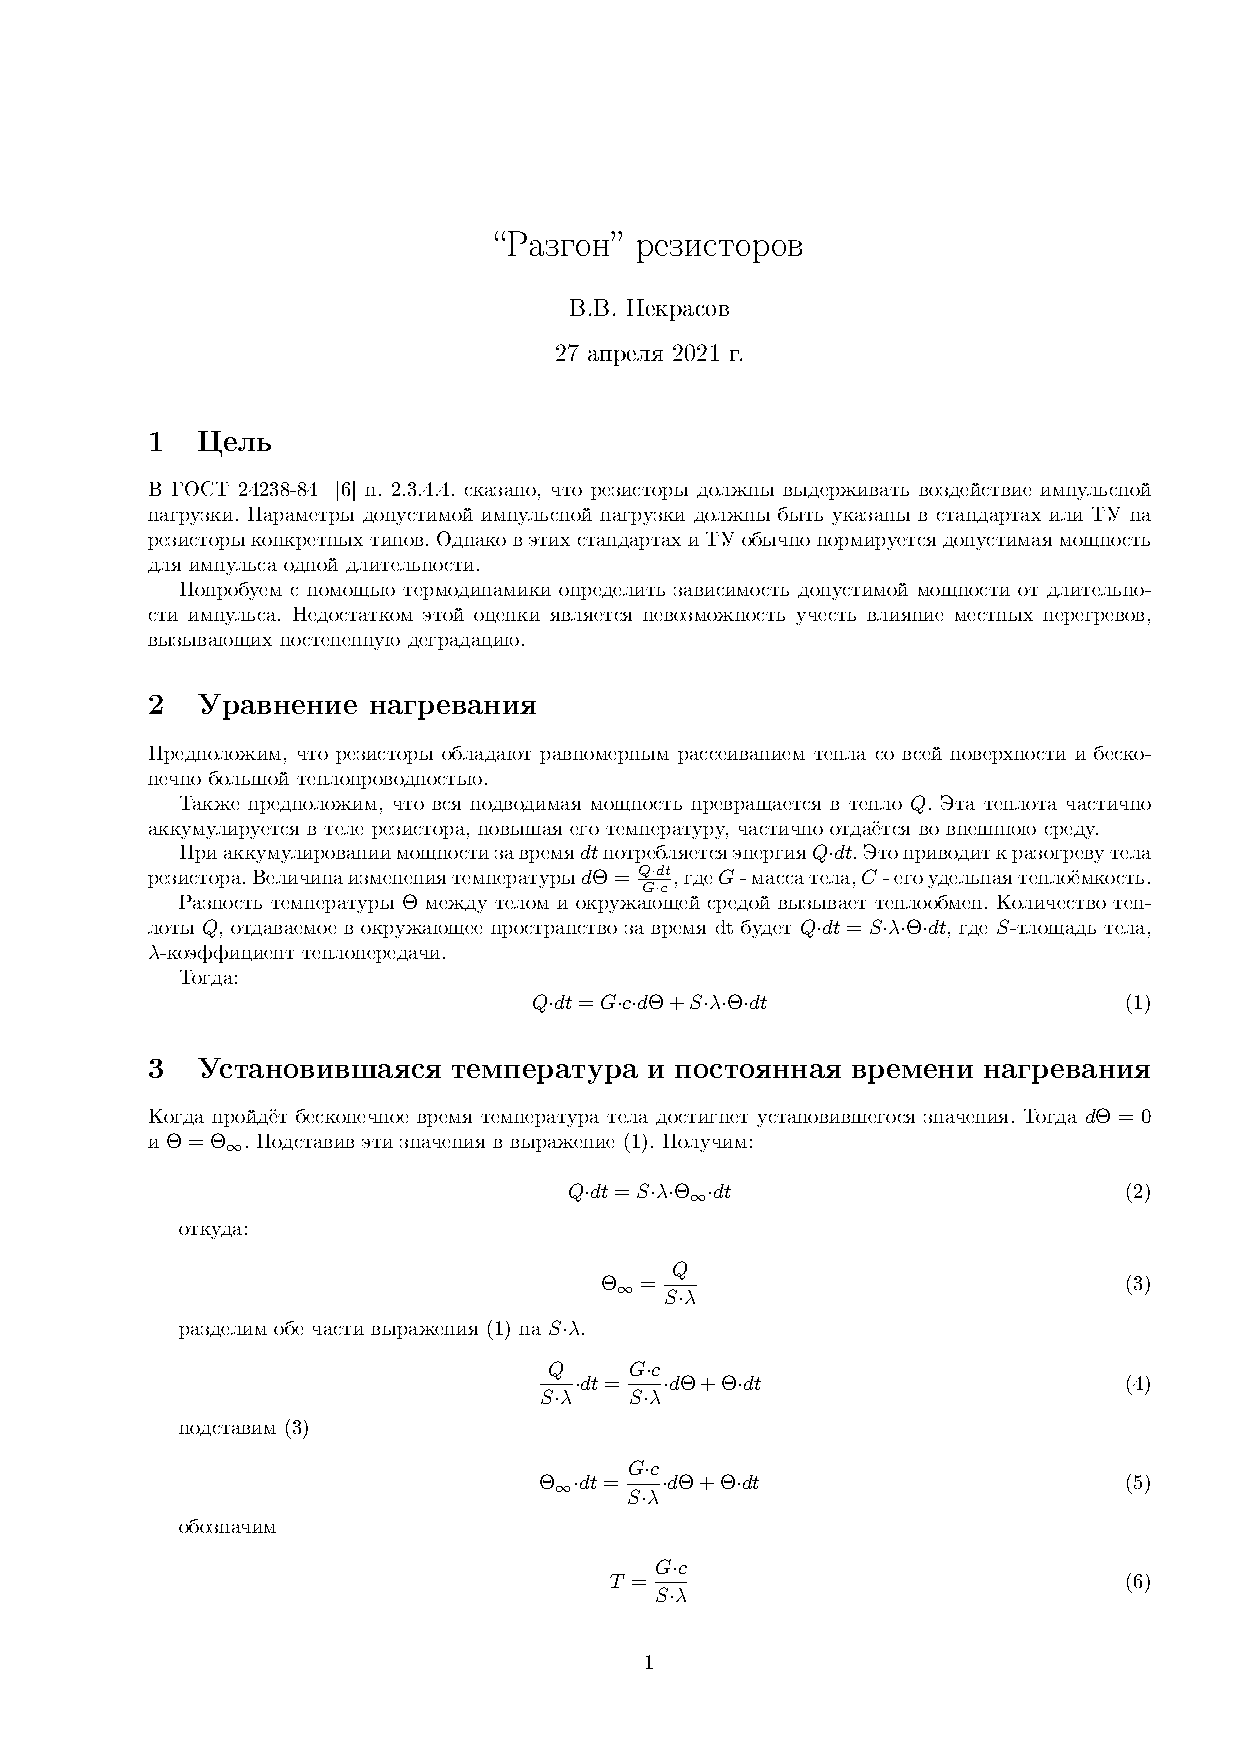
\includegraphics{Overclocking_resistors.png}

\begin{thebibliography}{2}
\bibitem{alyr.434110.005}
Резисторы постоянные непроволочные Р1-12. Технические условия АЛЯР.434110.005 ТУ

\bibitem{gost21342.14-86}
Резисторы методы испытания импульсной нагрузкой ГОСТ 21342.14-86

\bibitem{gost24238-84}
Резисторы постоянные общие технические условия ГОСТ 24238-84

\bibitem{heating_cooling}
Нагревание и охлаждение идеального однородного твердого тела.

URL: https://www.electromechanics.ru/direct-current/591-heating-and-cooling-is-ideal-homogeneous-solid.html
\end{thebibliography}

\end{document}
